\documentclass[11pt]{article}
\usepackage[margin=1in]{geometry}
\usepackage{enumitem}
\usepackage{hyperref}
\usepackage{graphicx}
\usepackage{array}
\usepackage{multicol}
\usepackage{longtable}
\usepackage{titlesec}
\usepackage{float}
\usepackage{amsmath}

\begin{document}

%==================================================
\begin{center}
\large \textbf{Sri Sivasubramaniya Nadar College of Engineering, Chennai} \\
(An Autonomous Institution Affiliated to Anna University) \\
\vspace{0.3cm}
\end{center}

\begin{table}[!h]
\renewcommand{\arraystretch}{1.5}
\resizebox{\textwidth}{!}{%
\begin{tabular}{|l|cll|}
\hline
Degree \& Branch & \multicolumn{1}{c|}{B.E. Computer Science \& Engineering} & Semester & VI \\ \hline
Subject Code \& Name & \multicolumn{3}{c|}{UCS2612 -- Machine Learning Algorithms Laboratory} \\ \hline
Academic Year & 2025--2026 (Even) & Batch & 2023--2027 \\ \hline
Name & PRANAV D & Register No. & 3122235001098 \\ \hline
Due Date & \multicolumn{3}{c|}{27 January 2026} \\ \hline
\end{tabular}
}
\end{table}

\begin{center}
\textbf{Experiment 3: Regression Analysis using Linear and Regularized Models}
\end{center}

%==================================================
\section*{1. Aim and Objective}
To comprehensively implement and evaluate linear regression and regularized regression models for predicting continuous target variables in financial loan applications. The experiment encompasses multiple objectives including baseline model development, advanced regularization techniques implementation, systematic hyperparameter optimization, comprehensive performance evaluation using multiple statistical metrics, and detailed analysis of model generalization capabilities. Additionally, the study investigates overfitting and underfitting phenomena, examines the bias-variance tradeoff inherent in different regularization approaches, and analyzes the impact of regularization on model interpretability and coefficient stability in the presence of multicollinearity.

%==================================================
\section*{2. Dataset Description}
This experiment utilizes a comprehensive real-world regression dataset focused on loan application predictions, where the primary objective is to accurately estimate the loan sanction amount based on applicant characteristics and financial indicators. The target variable is the \textbf{Loan Sanction Amount (USD)}, representing the actual amount approved by financial institutions for loan disbursement.

Dataset reference:
\begin{itemize}
\item Kaggle: \href{https://www.kaggle.com/datasets/phileinsophos/predict-loan-amount-data}{Predict Loan Amount Data}
\end{itemize}

The dataset comprises 30,000 loan application instances characterized by 24 diverse attributes encompassing both numerical and categorical features. Key numerical features include 'Income (USD)' representing the applicant's annual income, 'Loan Amount Request (USD)' indicating the desired loan amount, 'Credit Score' reflecting the applicant's creditworthiness (typically ranging from 300 to 850), 'Property Price' denoting the value of the property being financed, 'Property Age' in years, 'Current Loan Expenses (USD)', and 'Expense Type' categories. Categorical features include 'Gender', 'Property Location', 'Profession', 'Type of Employment', and 'Co-Applicant' status, among others.

This dataset presents several analytical challenges characteristic of real-world financial data, including potential multicollinearity among financial variables (particularly between income, property price, and loan request amounts), mixed data types requiring careful preprocessing, and inherent uncertainty in loan approval decisions influenced by institutional policies and economic conditions. The dataset's complexity and scale make it an ideal candidate for exploring the effectiveness of regularization techniques in managing feature interactions and improving model generalization.

%==================================================
\section*{3. Data Preprocessing Pipeline}
A systematic and rigorous preprocessing pipeline was implemented to ensure data quality and model readiness:

\subsection*{3.1 Missing Value Treatment}
\begin{itemize}
\item Conducted comprehensive missing value analysis across all 24 features
\item Implemented strategic imputation techniques:
\begin{itemize}
\item \textbf{Numerical features}: Applied mean imputation for features with missing values less than 5\%, preserving central tendency while minimizing bias
\item \textbf{Categorical features}: Employed mode imputation to replace missing values with the most frequent category, maintaining distribution characteristics
\item Features with excessive missing values (>30\%) were flagged for potential removal or separate analysis
\end{itemize}
\end{itemize}

\subsection*{3.2 Categorical Variable Encoding}
\begin{itemize}
\item Applied one-hot encoding transformation to categorical variables including 'Gender', 'Property Location', 'Profession', 'Type of Employment', and 'Co-Applicant' status
\item This encoding scheme creates binary dummy variables for each category, enabling linear models to process non-numerical data effectively
\item Implemented drop-first strategy to avoid multicollinearity from dummy variable trap, reducing dimensionality by one per categorical feature
\item Final encoded dataset expanded to incorporate all categorical information while maintaining numerical compatibility
\end{itemize}

\subsection*{3.3 Feature Standardization}
\begin{itemize}
\item Applied standardization (Z-score normalization) to all numerical features, transforming them to have zero mean and unit variance
\item Standardization is crucial for regularized regression models as it ensures that:
\begin{itemize}
\item Regularization penalties are applied uniformly across all features regardless of their original scales
\item Gradient descent optimization converges more efficiently and reliably
\item Model coefficients become directly comparable, facilitating feature importance interpretation
\end{itemize}
\item Used StandardScaler from scikit-learn, fitted on training data and applied to both training and testing sets to prevent data leakage
\end{itemize}

\subsection*{3.4 Data Partitioning}
\begin{itemize}
\item Split the dataset into training (80\%, 24,000 instances) and validation/testing (20\%, 6,000 instances) sets using stratified random sampling where applicable
\item The 80-20 split provides sufficient training data for model learning while reserving adequate samples for unbiased performance evaluation
\item Maintained consistent random seed for reproducibility across experiments
\end{itemize}

%==================================================
\section*{4. Theoretical Foundation}

\subsection*{4.1 Linear Regression}
Linear Regression establishes a linear relationship between input features $X$ and the continuous target variable $y$ through the equation:
\[
y = \beta_0 + \beta_1 x_1 + \beta_2 x_2 + \ldots + \beta_p x_p + \epsilon
\]

Where $\beta_0$ represents the intercept, $\beta_i$ denote feature coefficients, and $\epsilon$ captures residual error. The model minimizes the sum of squared residuals (Ordinary Least Squares criterion) to determine optimal parameter values. Linear regression serves as an interpretable baseline model but is susceptible to overfitting when features are highly correlated (multicollinearity) or when the number of features approaches the number of observations.

\subsection*{4.2 Regularized Regression Models}
Regularization techniques introduce penalty terms to the loss function to constrain model complexity and improve generalization:

\subsubsection*{Ridge Regression (L2 Regularization)}
Ridge regression adds an L2 penalty term proportional to the sum of squared coefficients:
\[
\text{Loss} = \sum_{i=1}^{n} (y_i - \hat{y}_i)^2 + \alpha \sum_{j=1}^{p} \beta_j^2
\]

The hyperparameter $\alpha$ controls regularization strength. Ridge regression shrinks coefficient magnitudes toward zero but never eliminates features entirely. It is particularly effective when features exhibit multicollinearity, as it distributes coefficient weights across correlated features rather than arbitrarily selecting one.

\subsubsection*{Lasso Regression (L1 Regularization)}
Lasso (Least Absolute Shrinkage and Selection Operator) employs an L1 penalty term:
\[
\text{Loss} = \sum_{i=1}^{n} (y_i - \hat{y}_i)^2 + \alpha \sum_{j=1}^{p} |\beta_j|
\]

The L1 penalty induces sparsity by driving some coefficients exactly to zero, effectively performing automatic feature selection. This property makes Lasso particularly valuable for high-dimensional datasets where identifying relevant features is crucial. However, when features are highly correlated, Lasso tends to select one arbitrarily and ignore others.

\subsubsection*{Elastic Net Regression (Combined L1 + L2)}
Elastic Net combines the strengths of Ridge and Lasso through a hybrid penalty:
\[
\text{Loss} = \sum_{i=1}^{n} (y_i - \hat{y}_i)^2 + \alpha \left( (1-\rho) \sum_{j=1}^{p} \beta_j^2 + \rho \sum_{j=1}^{p} |\beta_j| \right)
\]

Where $\rho$ (l1\_ratio) balances between L1 and L2 penalties. Elastic Net mitigates limitations of both Ridge and Lasso: it performs feature selection like Lasso while maintaining Ridge's ability to handle correlated features. This makes it particularly suitable for real-world datasets with complex feature interactions.

\subsection*{4.3 Regularization Benefits}
Regularization techniques provide multiple advantages:
\begin{itemize}
\item \textbf{Overfitting Prevention}: Constrains model complexity, reducing sensitivity to training data noise
\item \textbf{Improved Generalization}: Enhances performance on unseen data by preventing memorization of training patterns
\item \textbf{Multicollinearity Management}: Stabilizes coefficient estimates when features are highly correlated
\item \textbf{Feature Selection}: Lasso and Elastic Net identify and eliminate irrelevant features
\item \textbf{Computational Stability}: Regularization improves numerical conditioning of optimization problems
\end{itemize}

%==================================================
\section*{5. Implementation Methodology}

\subsection*{5.1 Experimental Workflow}
The experimental procedure followed a systematic approach to ensure rigorous evaluation:

\begin{enumerate}[label=\arabic*.]
\item \textbf{Data Acquisition}: Loaded the comprehensive loan amount dataset from Kaggle repository

\item \textbf{Data Preprocessing}:
\begin{itemize}
\item Conducted exploratory data analysis to understand feature distributions and relationships
\item Identified and handled missing values through strategic imputation
\item Encoded categorical variables using one-hot encoding with dummy variable elimination
\item Standardized all numerical features to ensure uniform scale and facilitate regularization
\end{itemize}

\item \textbf{Exploratory Data Analysis (EDA)}:
\begin{itemize}
\item Visualized target variable distribution to assess normality and identify potential outliers
\item Generated correlation matrices to identify multicollinearity among features
\item Analyzed feature-target relationships through scatter plots and statistical measures
\item Examined feature distributions for skewness and unusual patterns
\end{itemize}

\item \textbf{Data Partitioning}: Split dataset into training (80\%) and testing (20\%) subsets with consistent random seed

\item \textbf{Baseline Model Development}: Trained standard Linear Regression without regularization to establish performance benchmark

\item \textbf{Regularized Model Training}: Implemented Ridge, Lasso, and Elastic Net regression variants

\item \textbf{Hyperparameter Optimization}:
\begin{itemize}
\item Performed 5-fold cross-validation for robust parameter selection
\item Employed Grid Search to exhaustively evaluate predefined hyperparameter spaces
\item Identified optimal regularization strengths ($\alpha$) and mixing parameters (l1\_ratio for Elastic Net)
\end{itemize}

\item \textbf{Comprehensive Model Evaluation}:
\begin{itemize}
\item Assessed all models using multiple regression metrics on both validation and test sets
\item Generated learning curves to analyze training dynamics and generalization behavior
\item Compared coefficient values across models to understand regularization effects
\item Visualized predictions against actual values and examined residual patterns
\end{itemize}
\end{enumerate}

%==================================================
\section*{6. Visualizations}

\subsection*{6.1 Exploratory Data Analysis}
\begin{figure}[H]
\centering
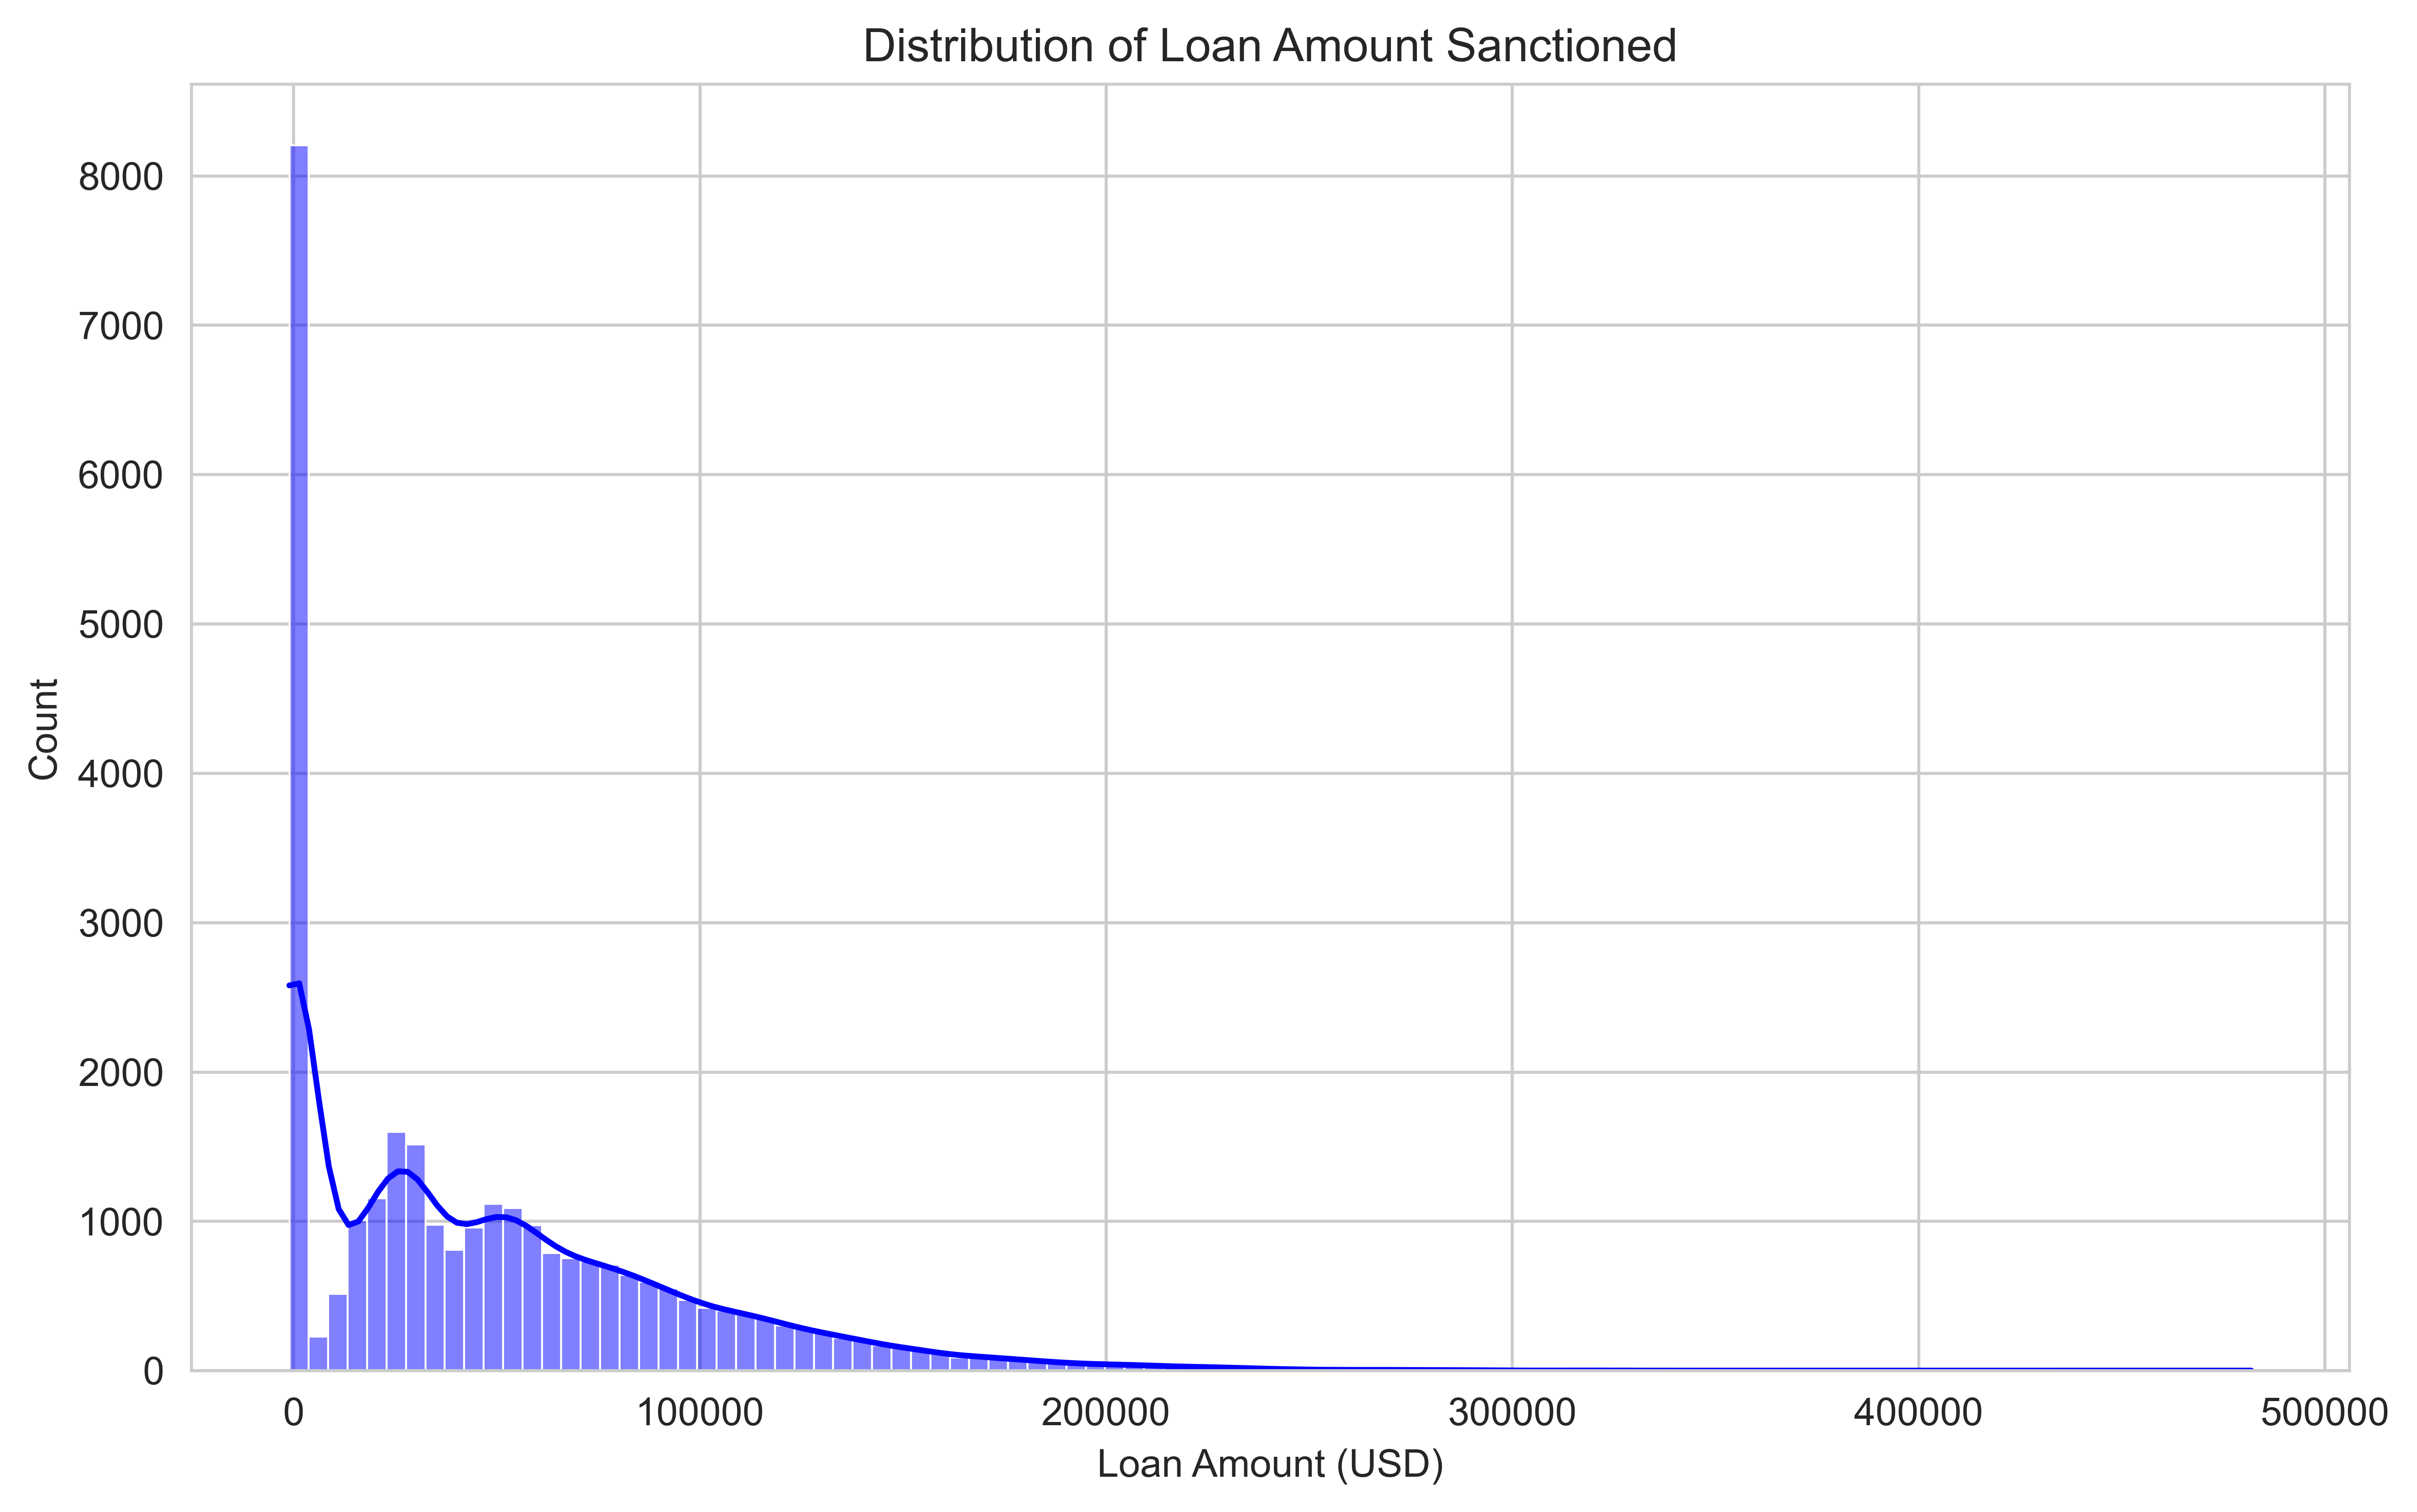
\includegraphics[width=0.7\textwidth]{png/target_distribution.png}
\caption{Distribution of Loan Sanction Amount (Target Variable)}
\end{figure}

\begin{figure}[H]
\centering
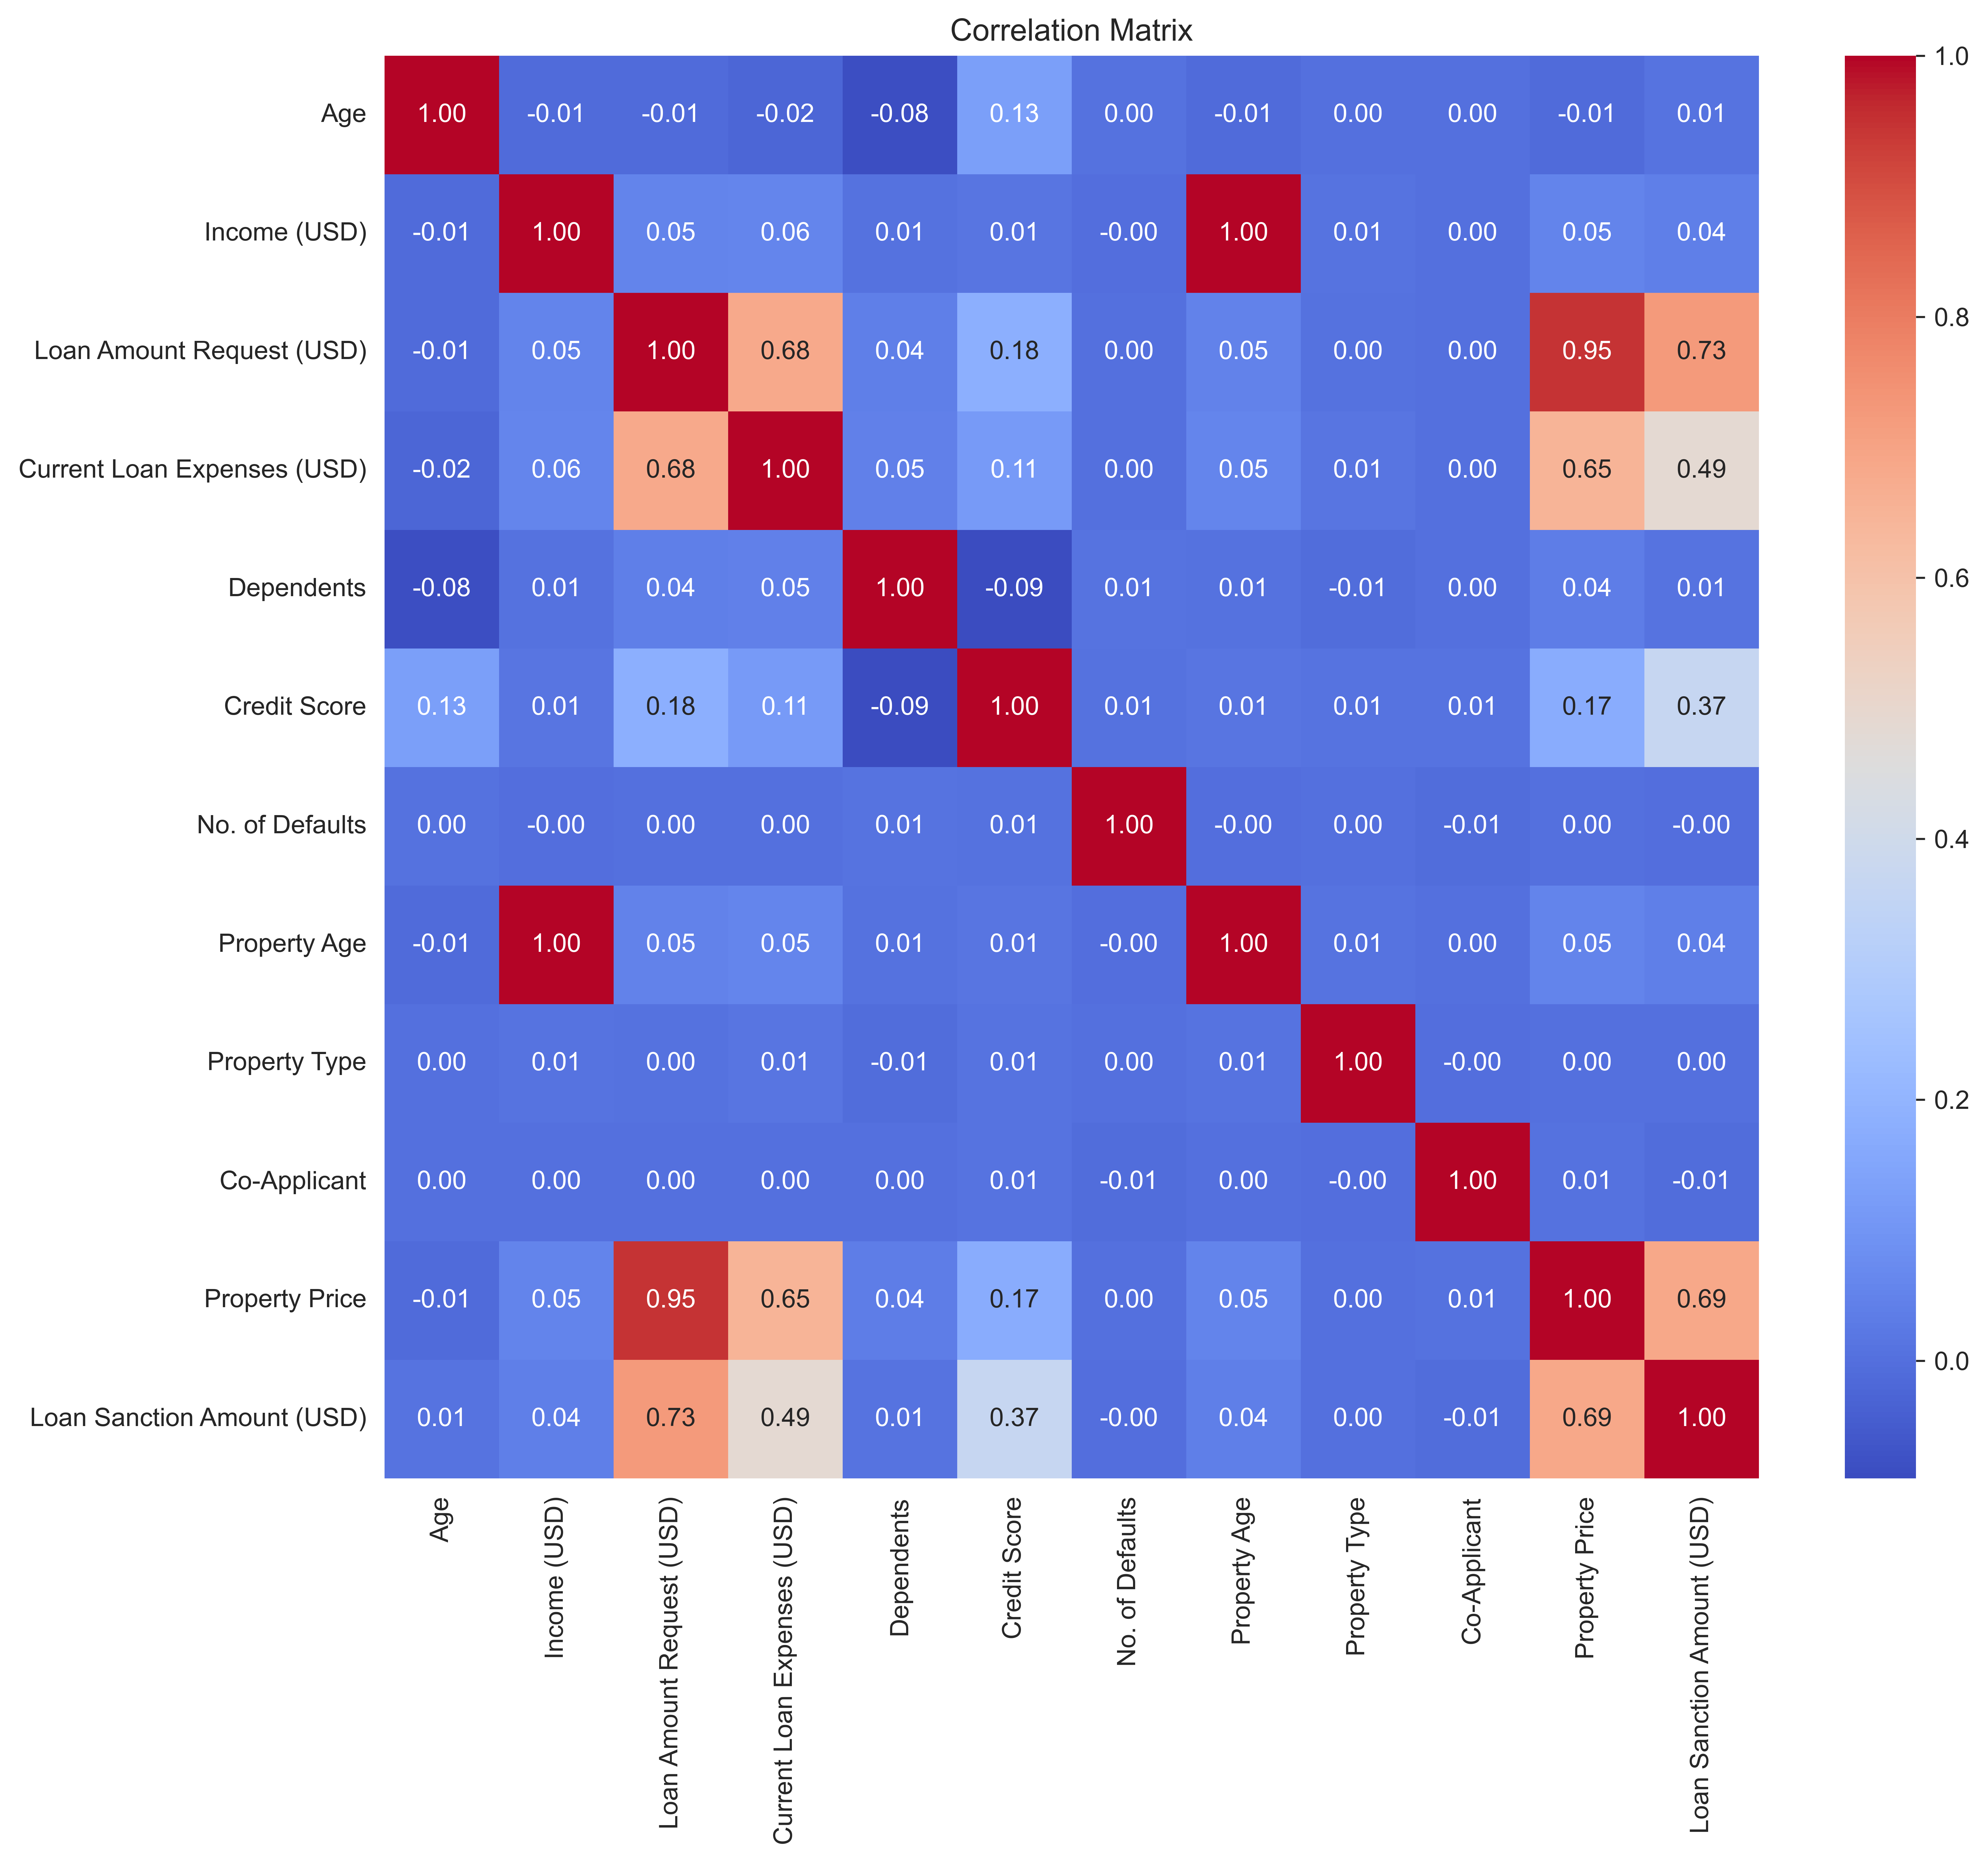
\includegraphics[width=0.8\textwidth]{png/correlation_heatmap.png}
\caption{Feature Correlation Heatmap Revealing Multicollinearity}
\end{figure}

\subsection*{6.2 Model Performance Evaluation}
\begin{figure}[H]
\centering
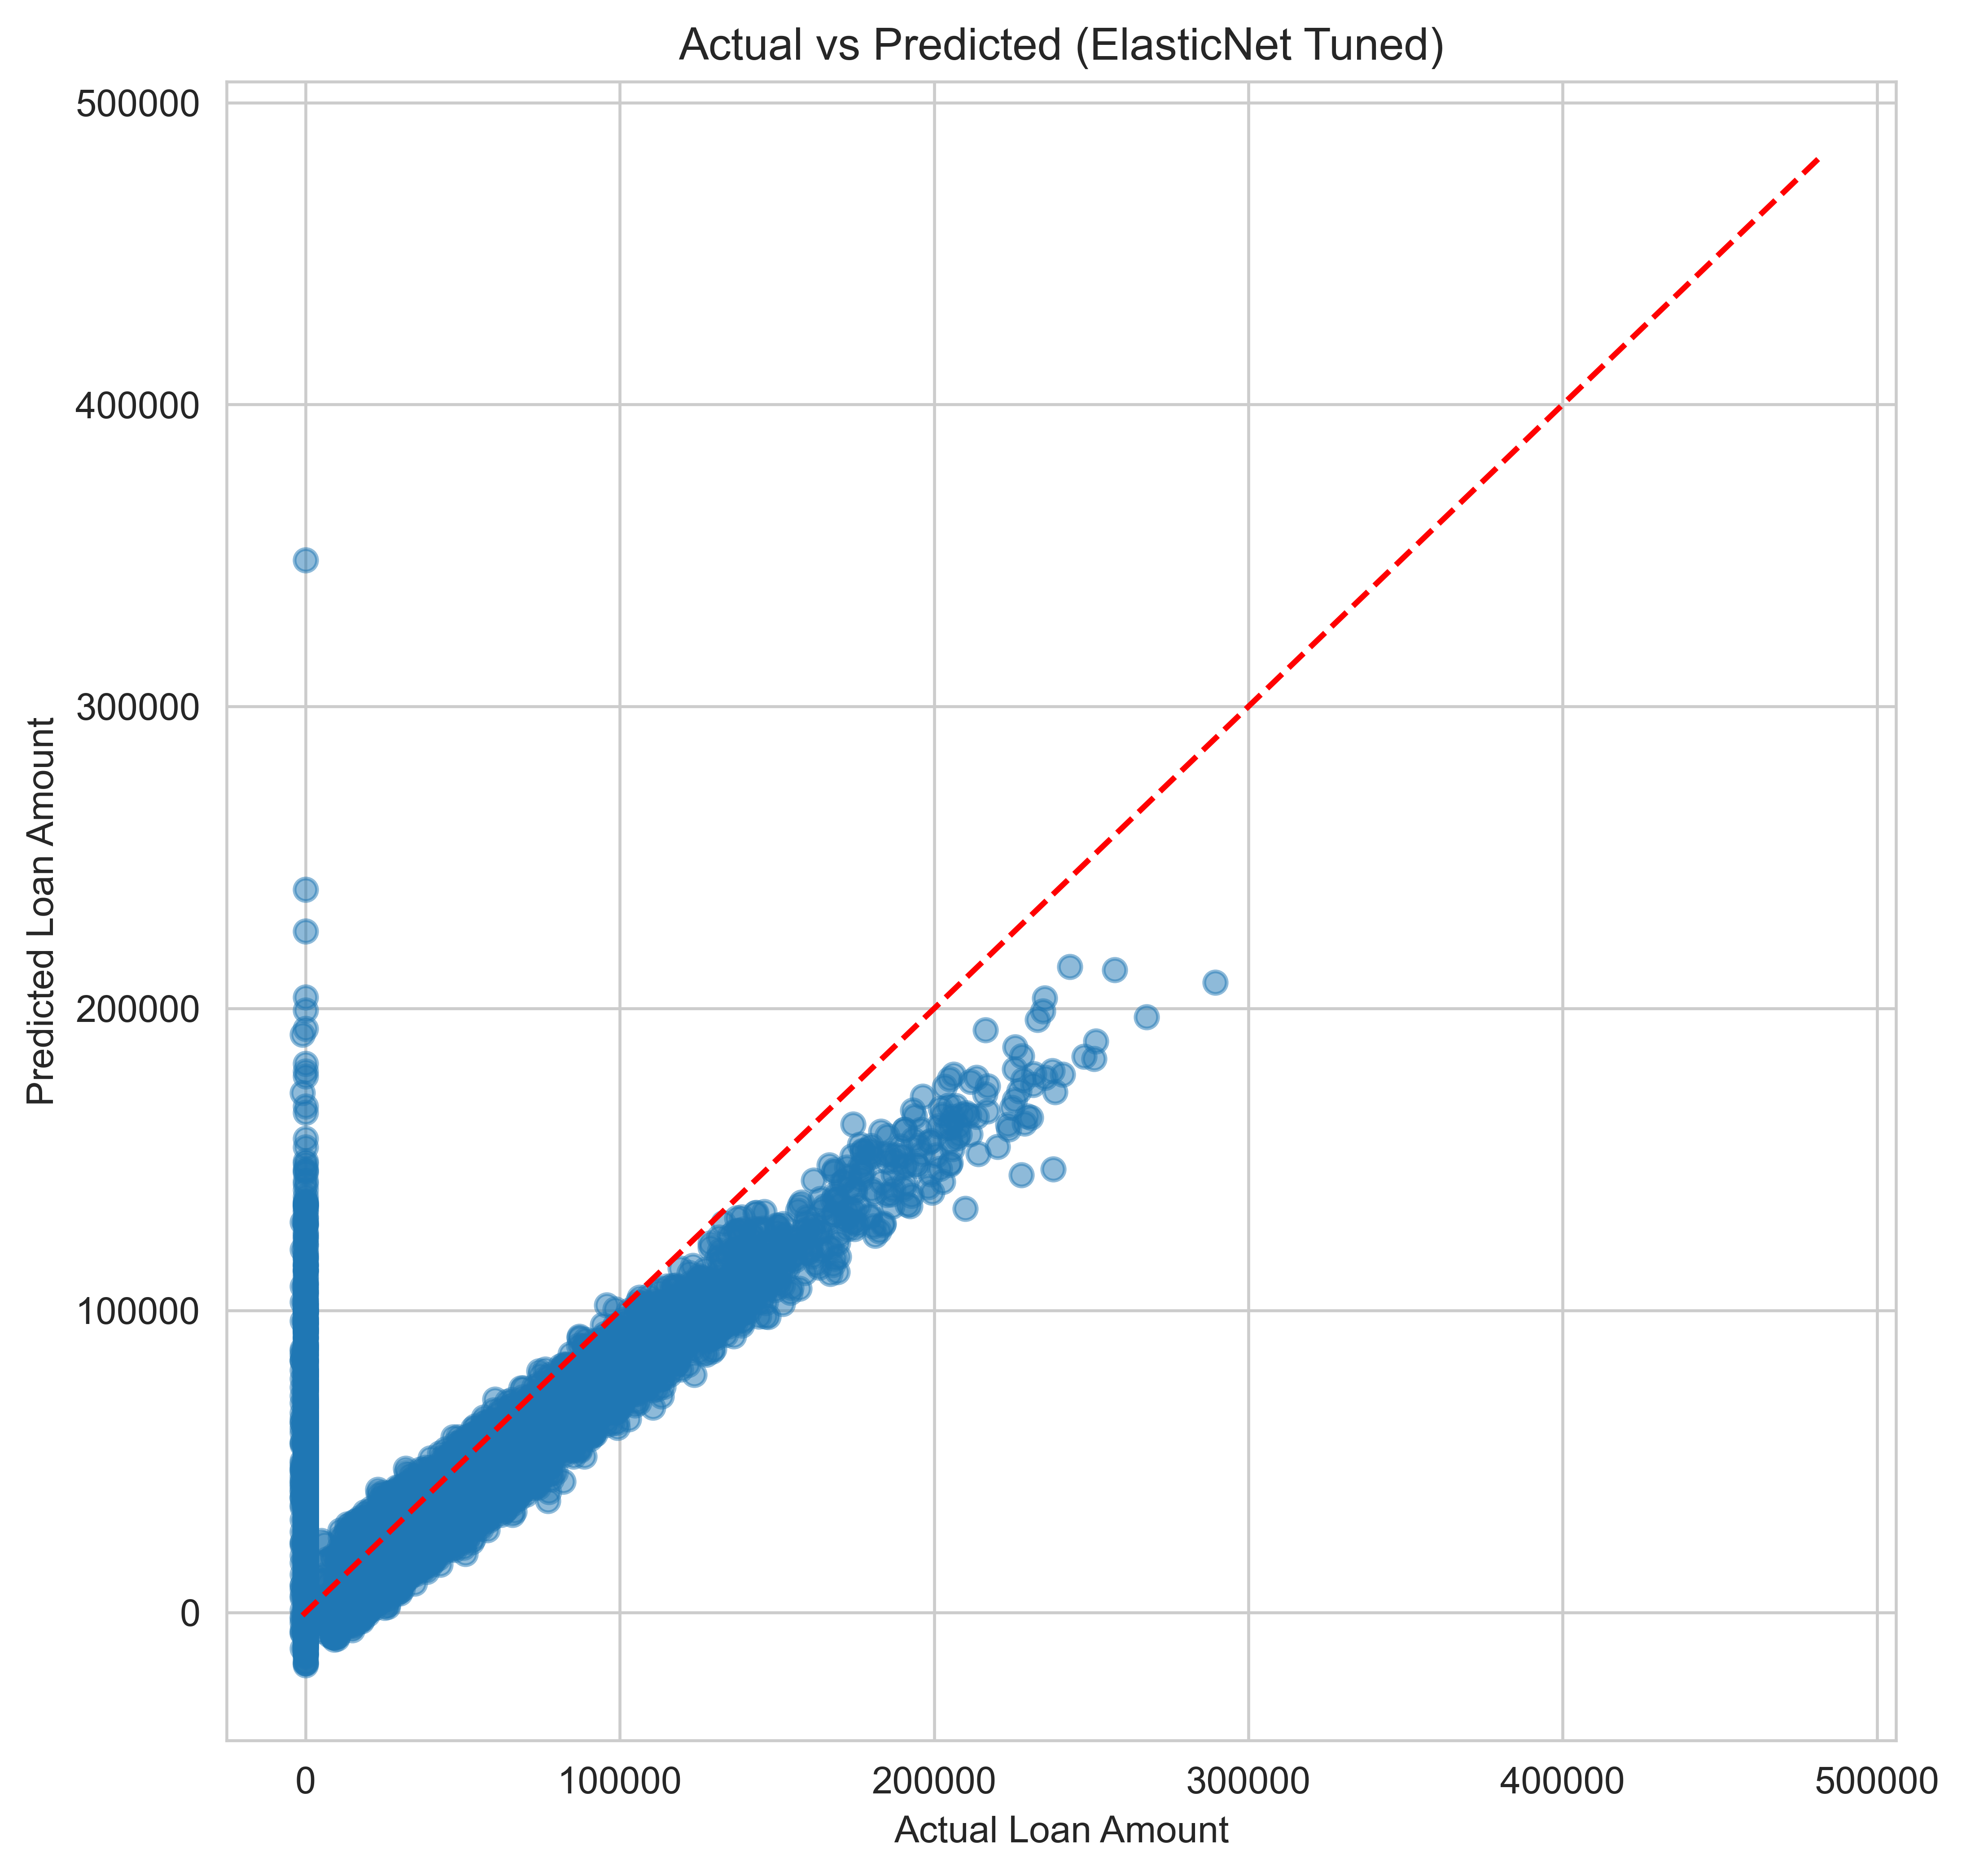
\includegraphics[width=0.6\textwidth]{png/predicted_vs_actual.png}
\caption{Predicted vs Actual Loan Amounts (Best Performing Model)}
\end{figure}

\begin{figure}[H]
\centering
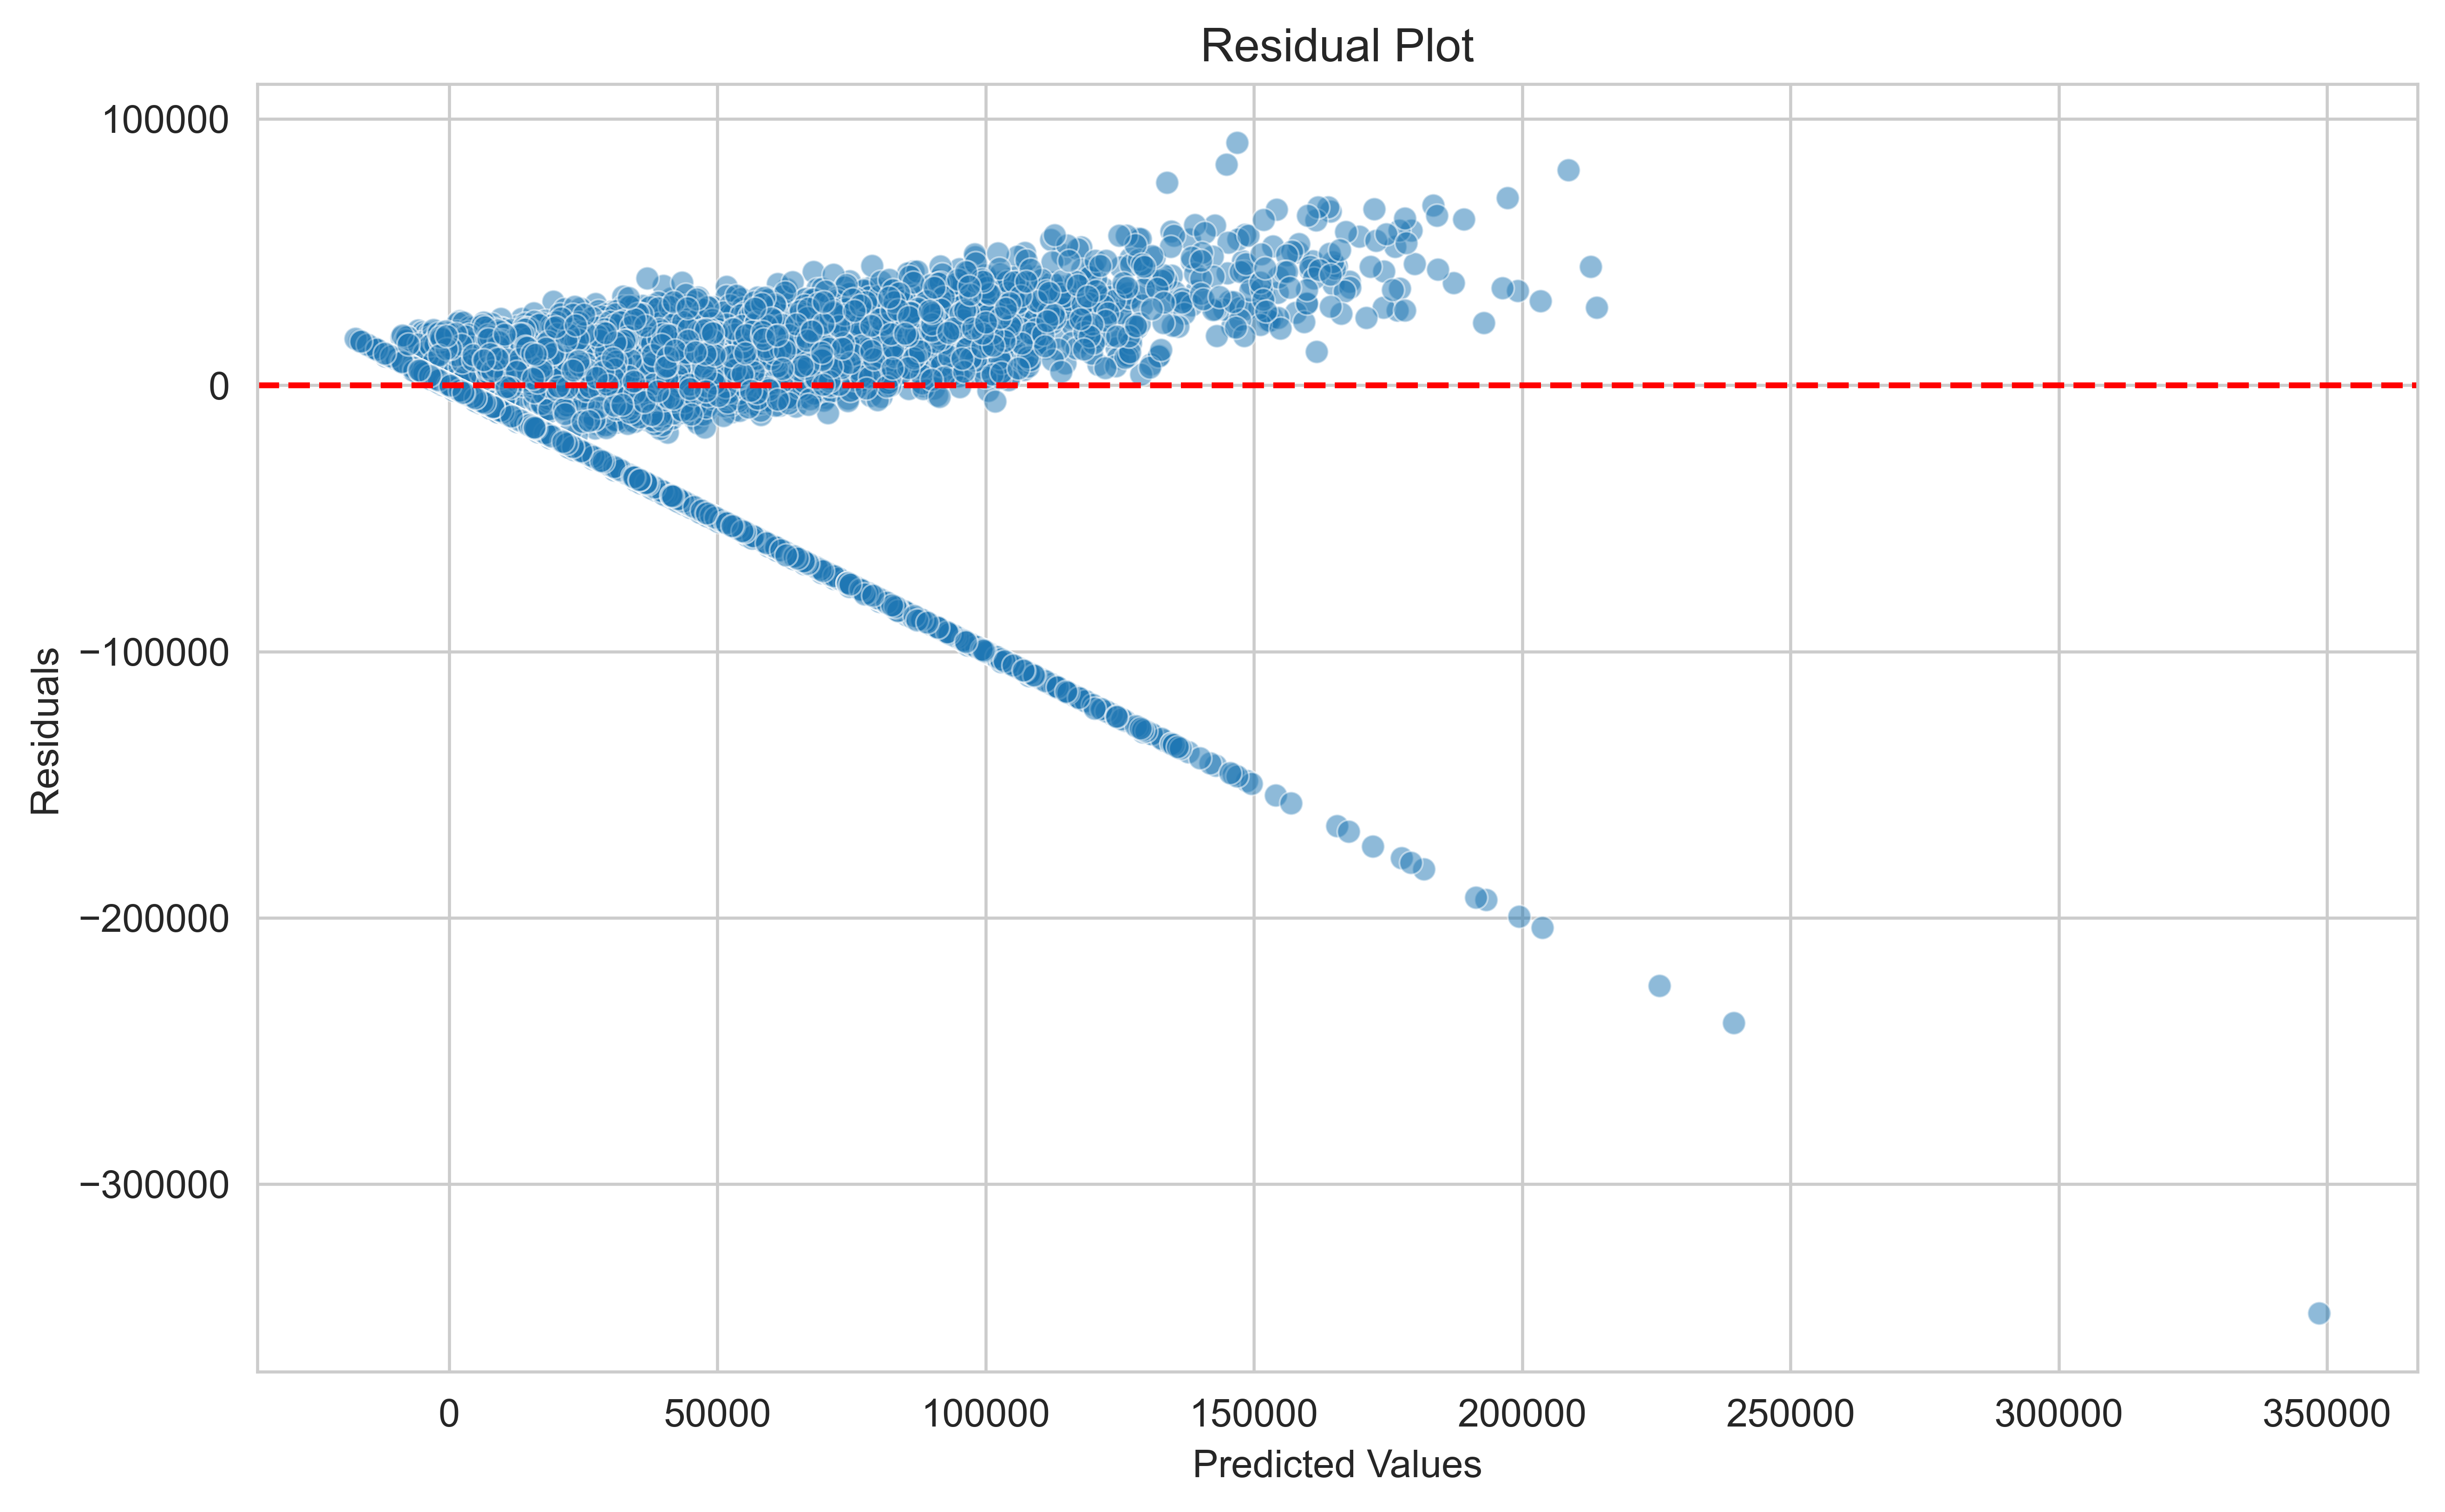
\includegraphics[width=0.7\textwidth]{png/residual_plot.png}
\caption{Residual Distribution Analysis for Model Diagnostics}
\end{figure}

\subsection*{6.3 Learning Curve Analysis}
\begin{figure}[H]
\centering
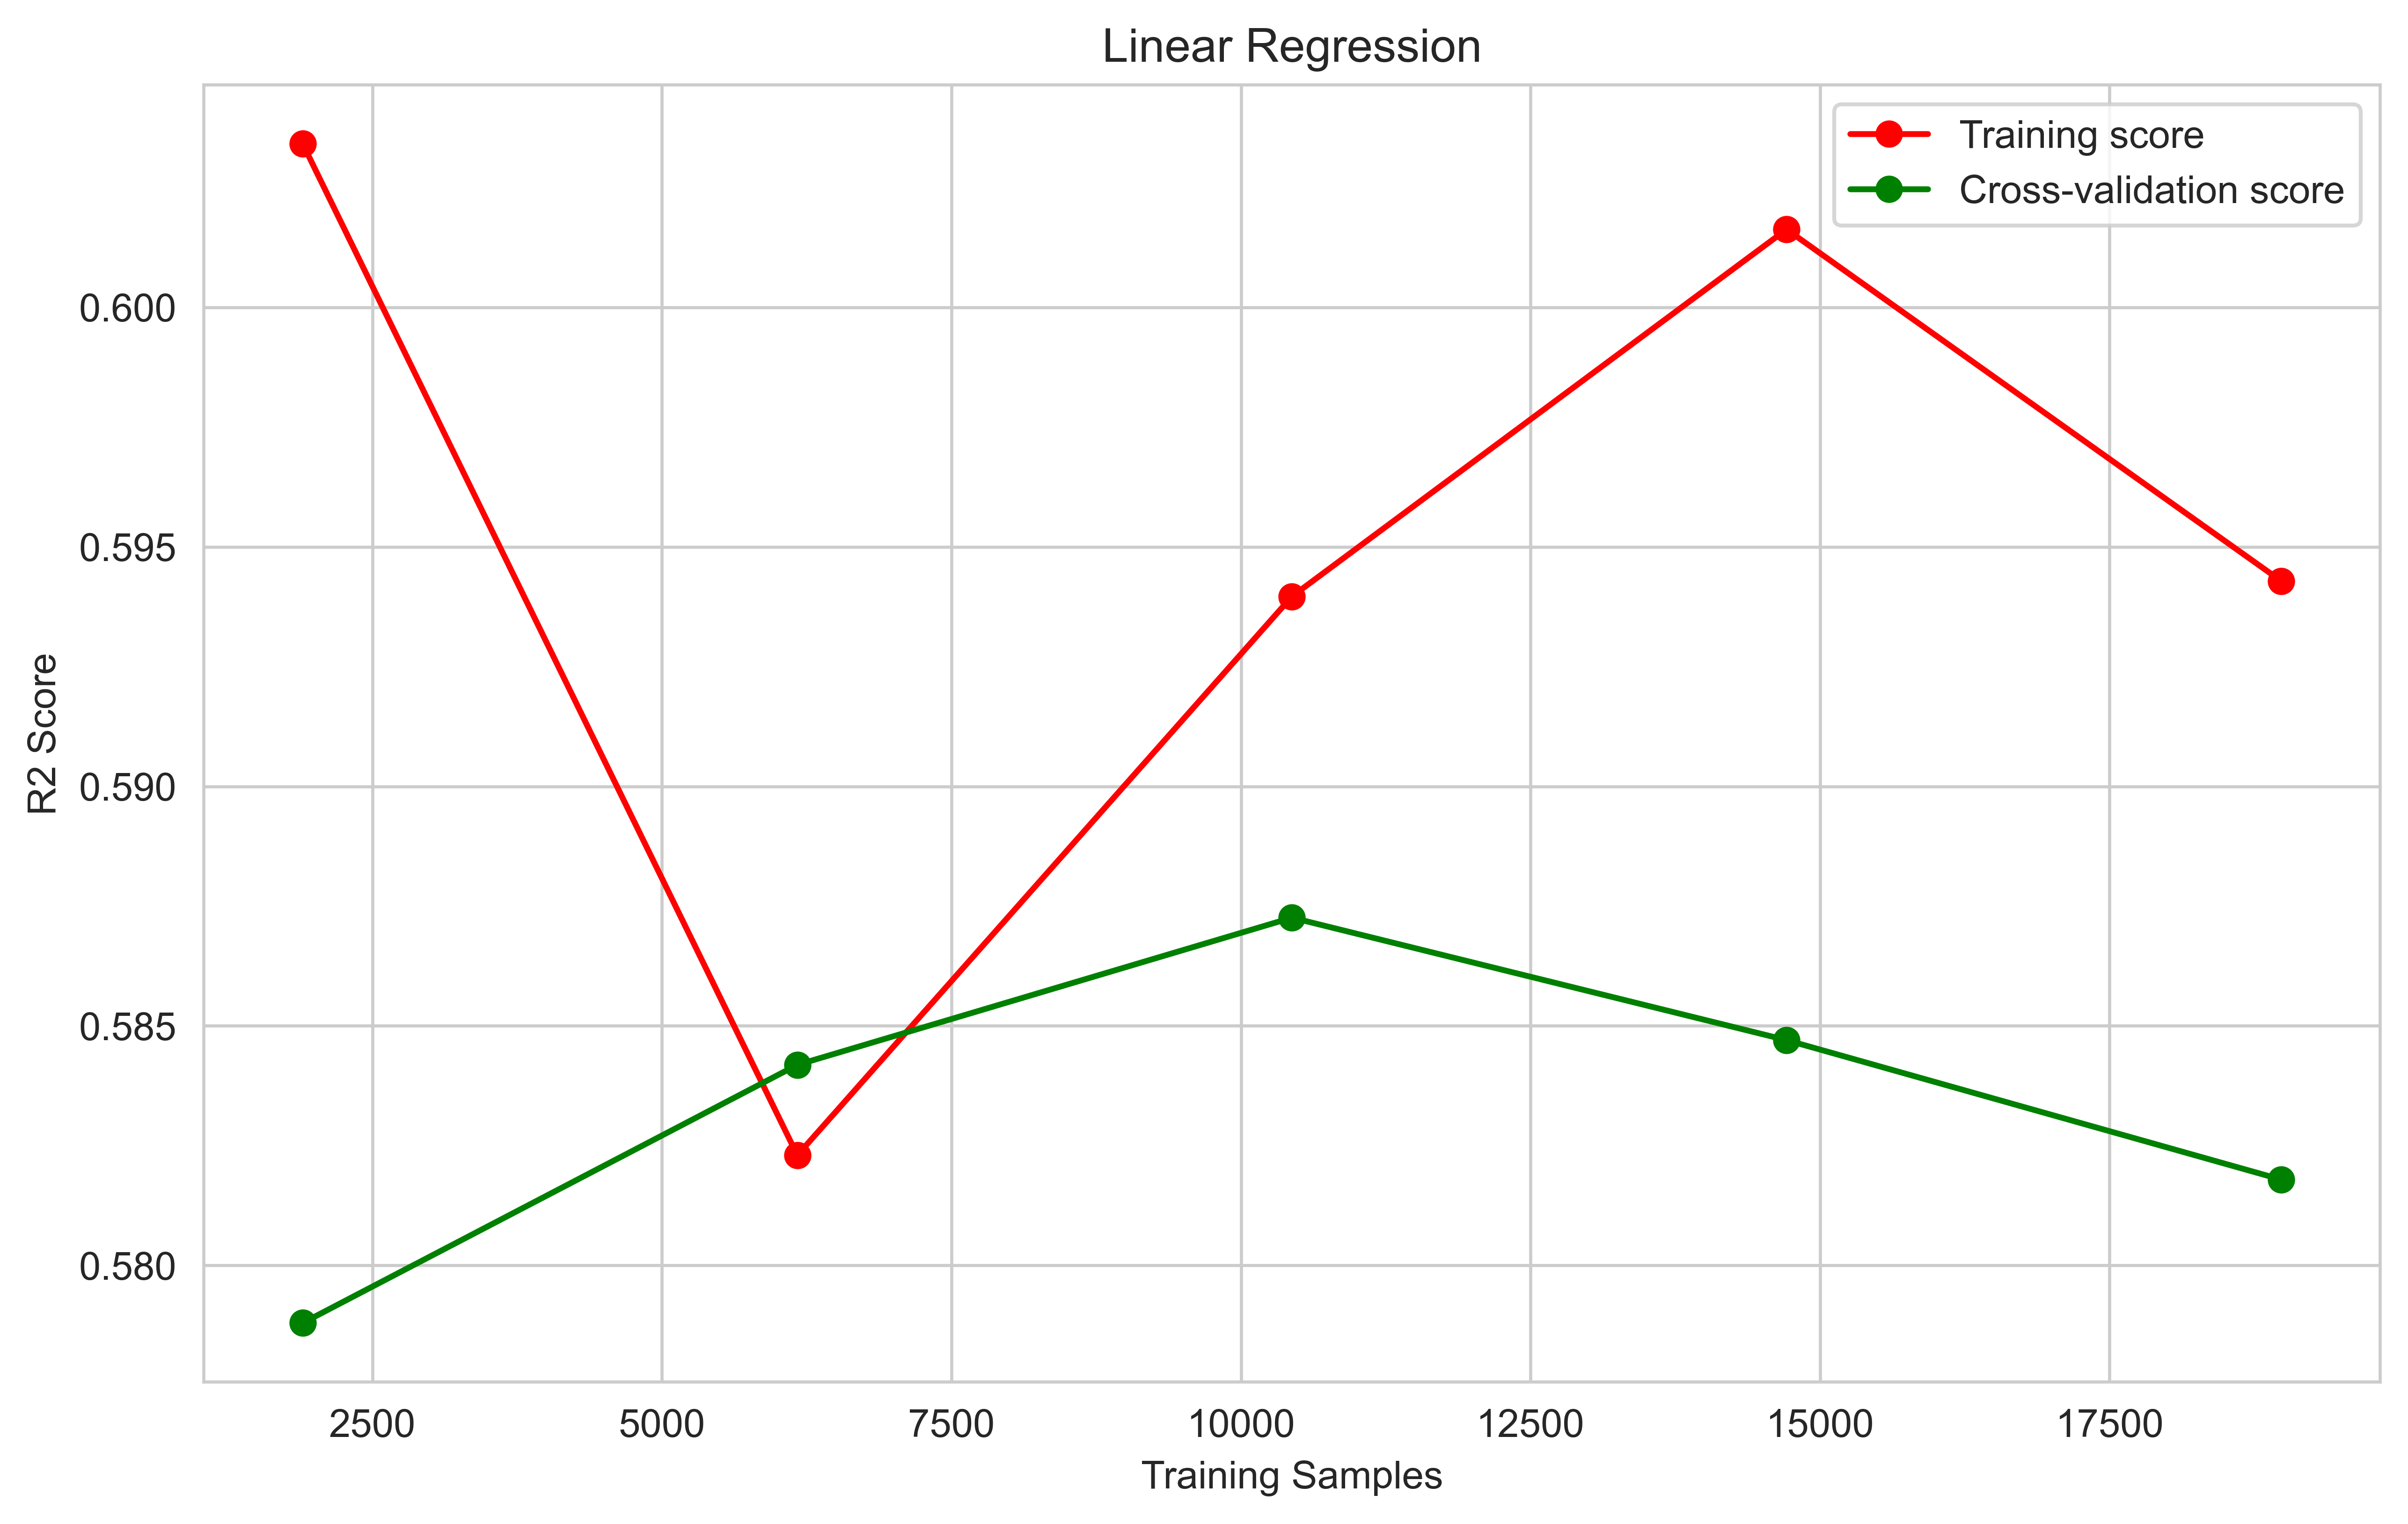
\includegraphics[width=0.7\textwidth]{png/learning_curve_Linear_Regression.png}
\caption{Learning Curve - Linear Regression}
\end{figure}

\begin{figure}[H]
\centering
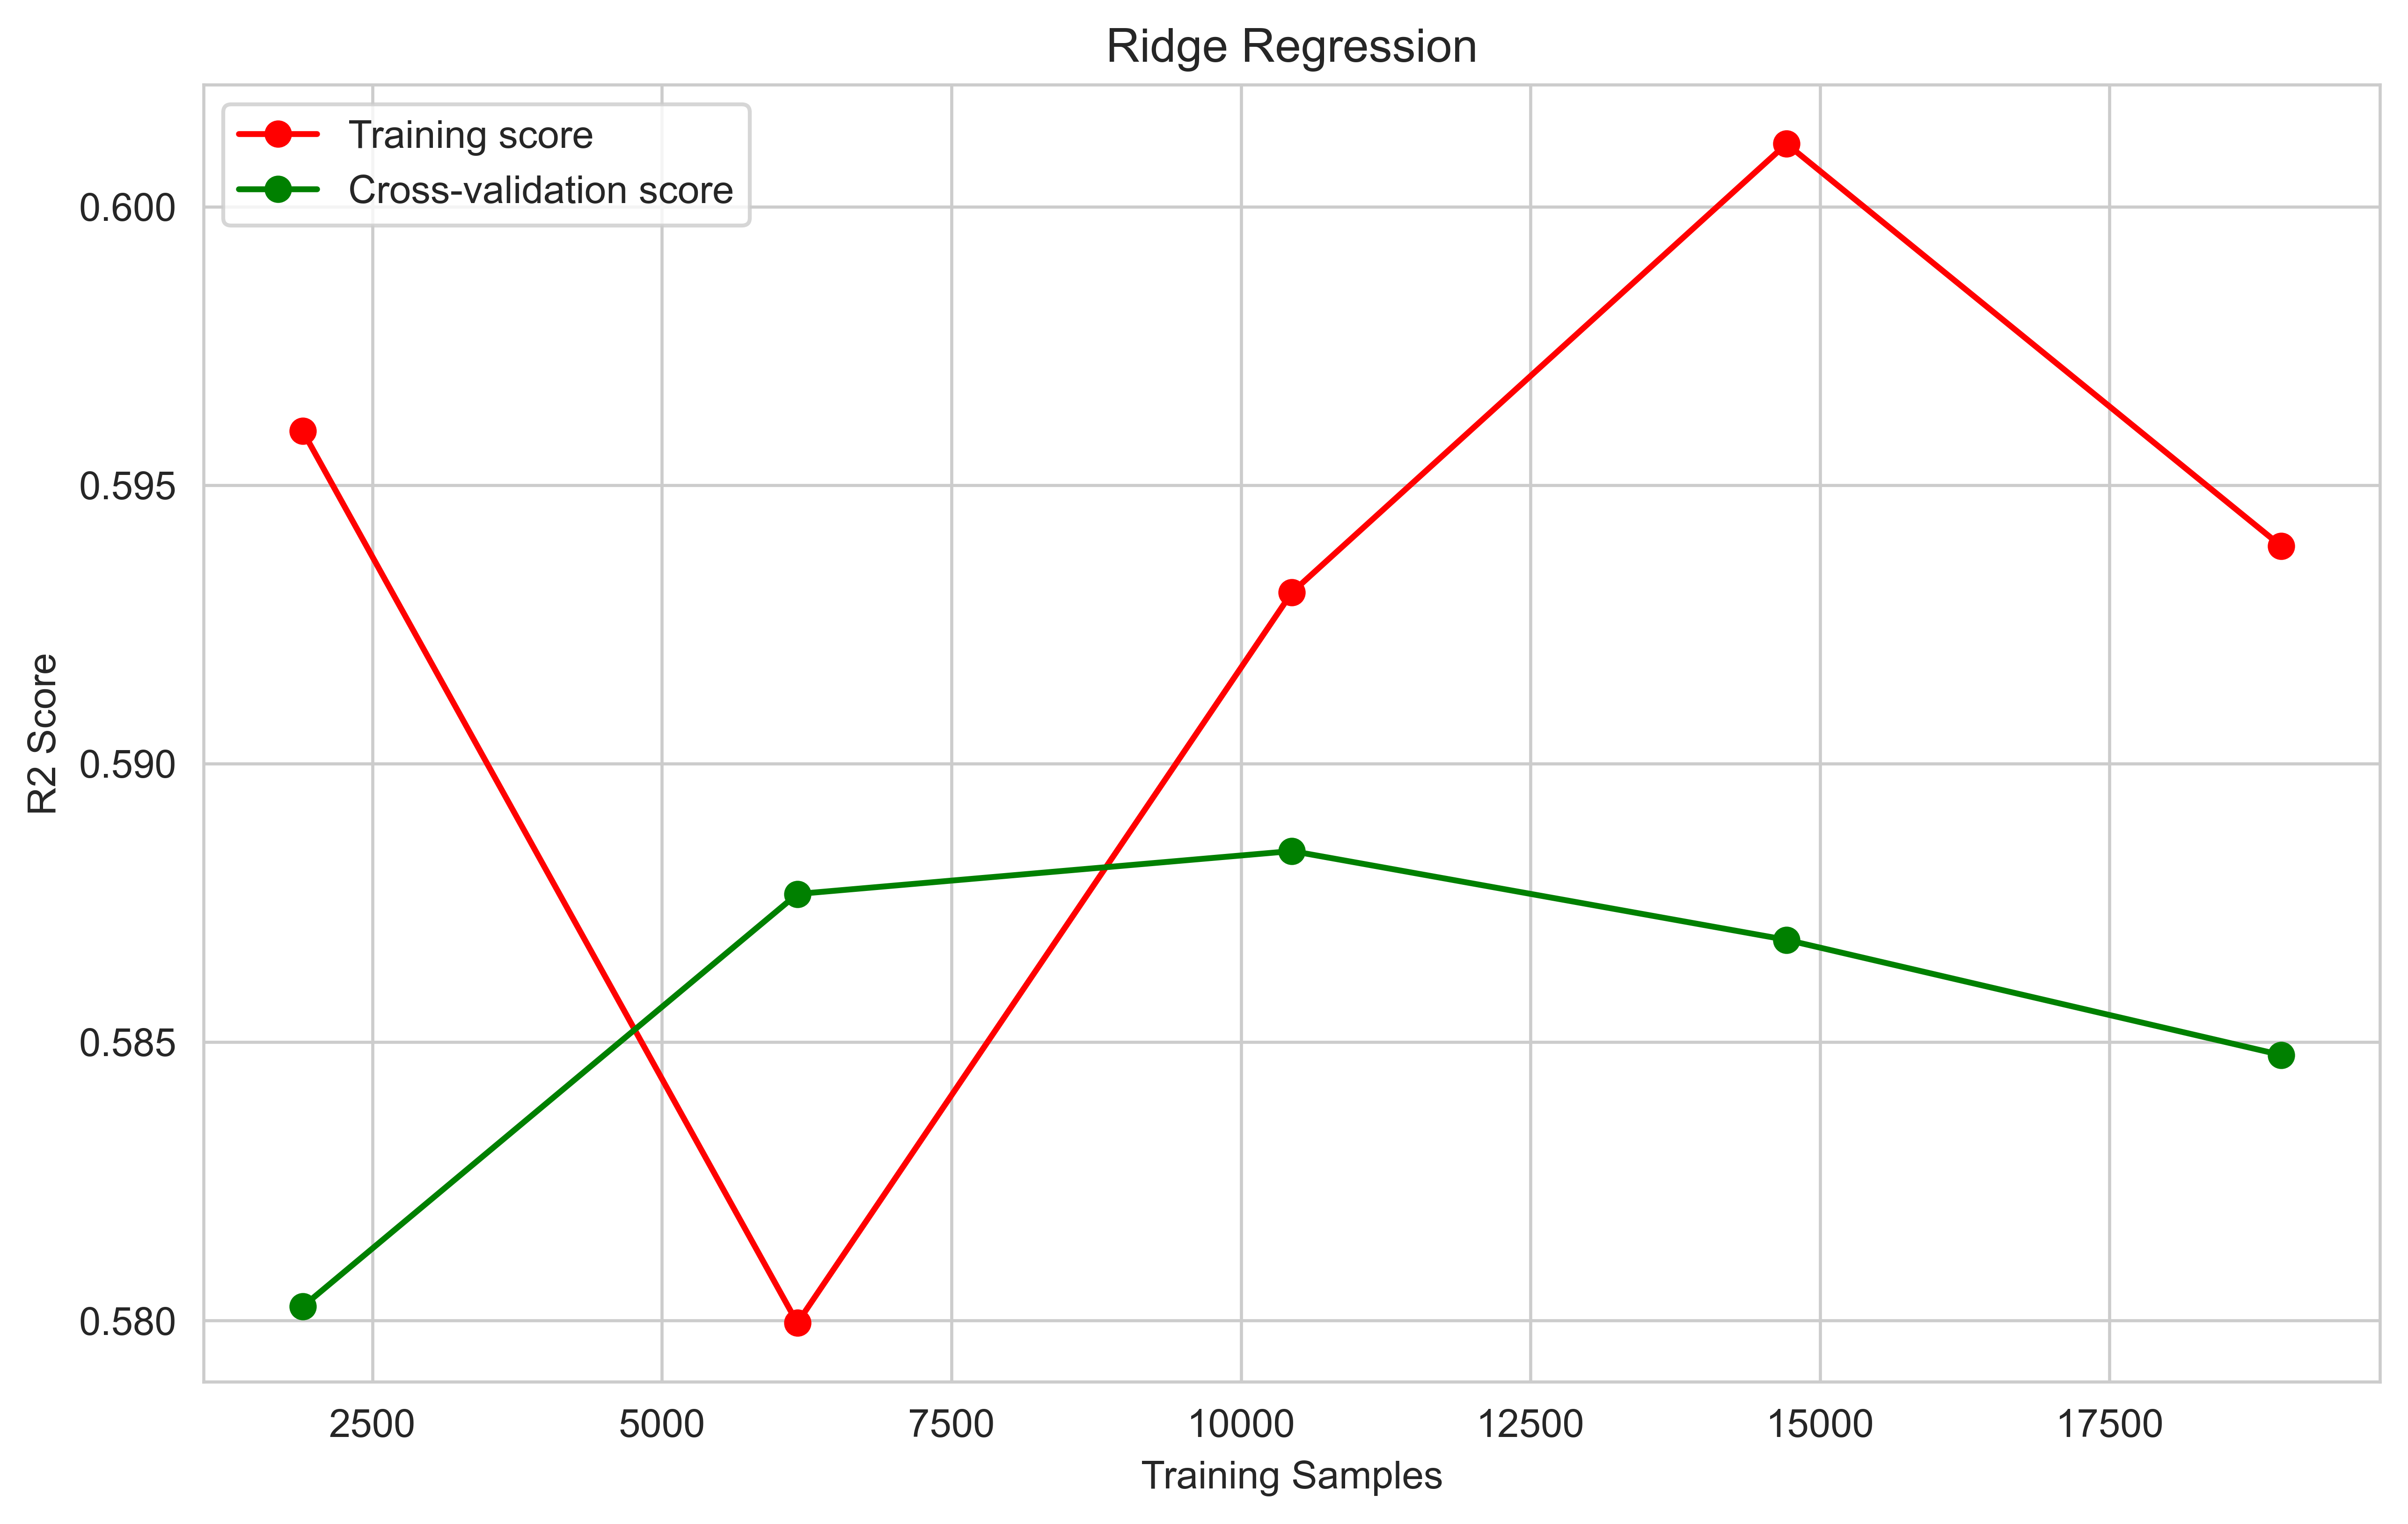
\includegraphics[width=0.7\textwidth]{png/learning_curve_Ridge_Regression.png}
\caption{Learning Curve - Ridge Regression with Regularization}
\end{figure}

\subsection*{6.4 Regularization Impact on Coefficients}
\begin{figure}[H]
\centering
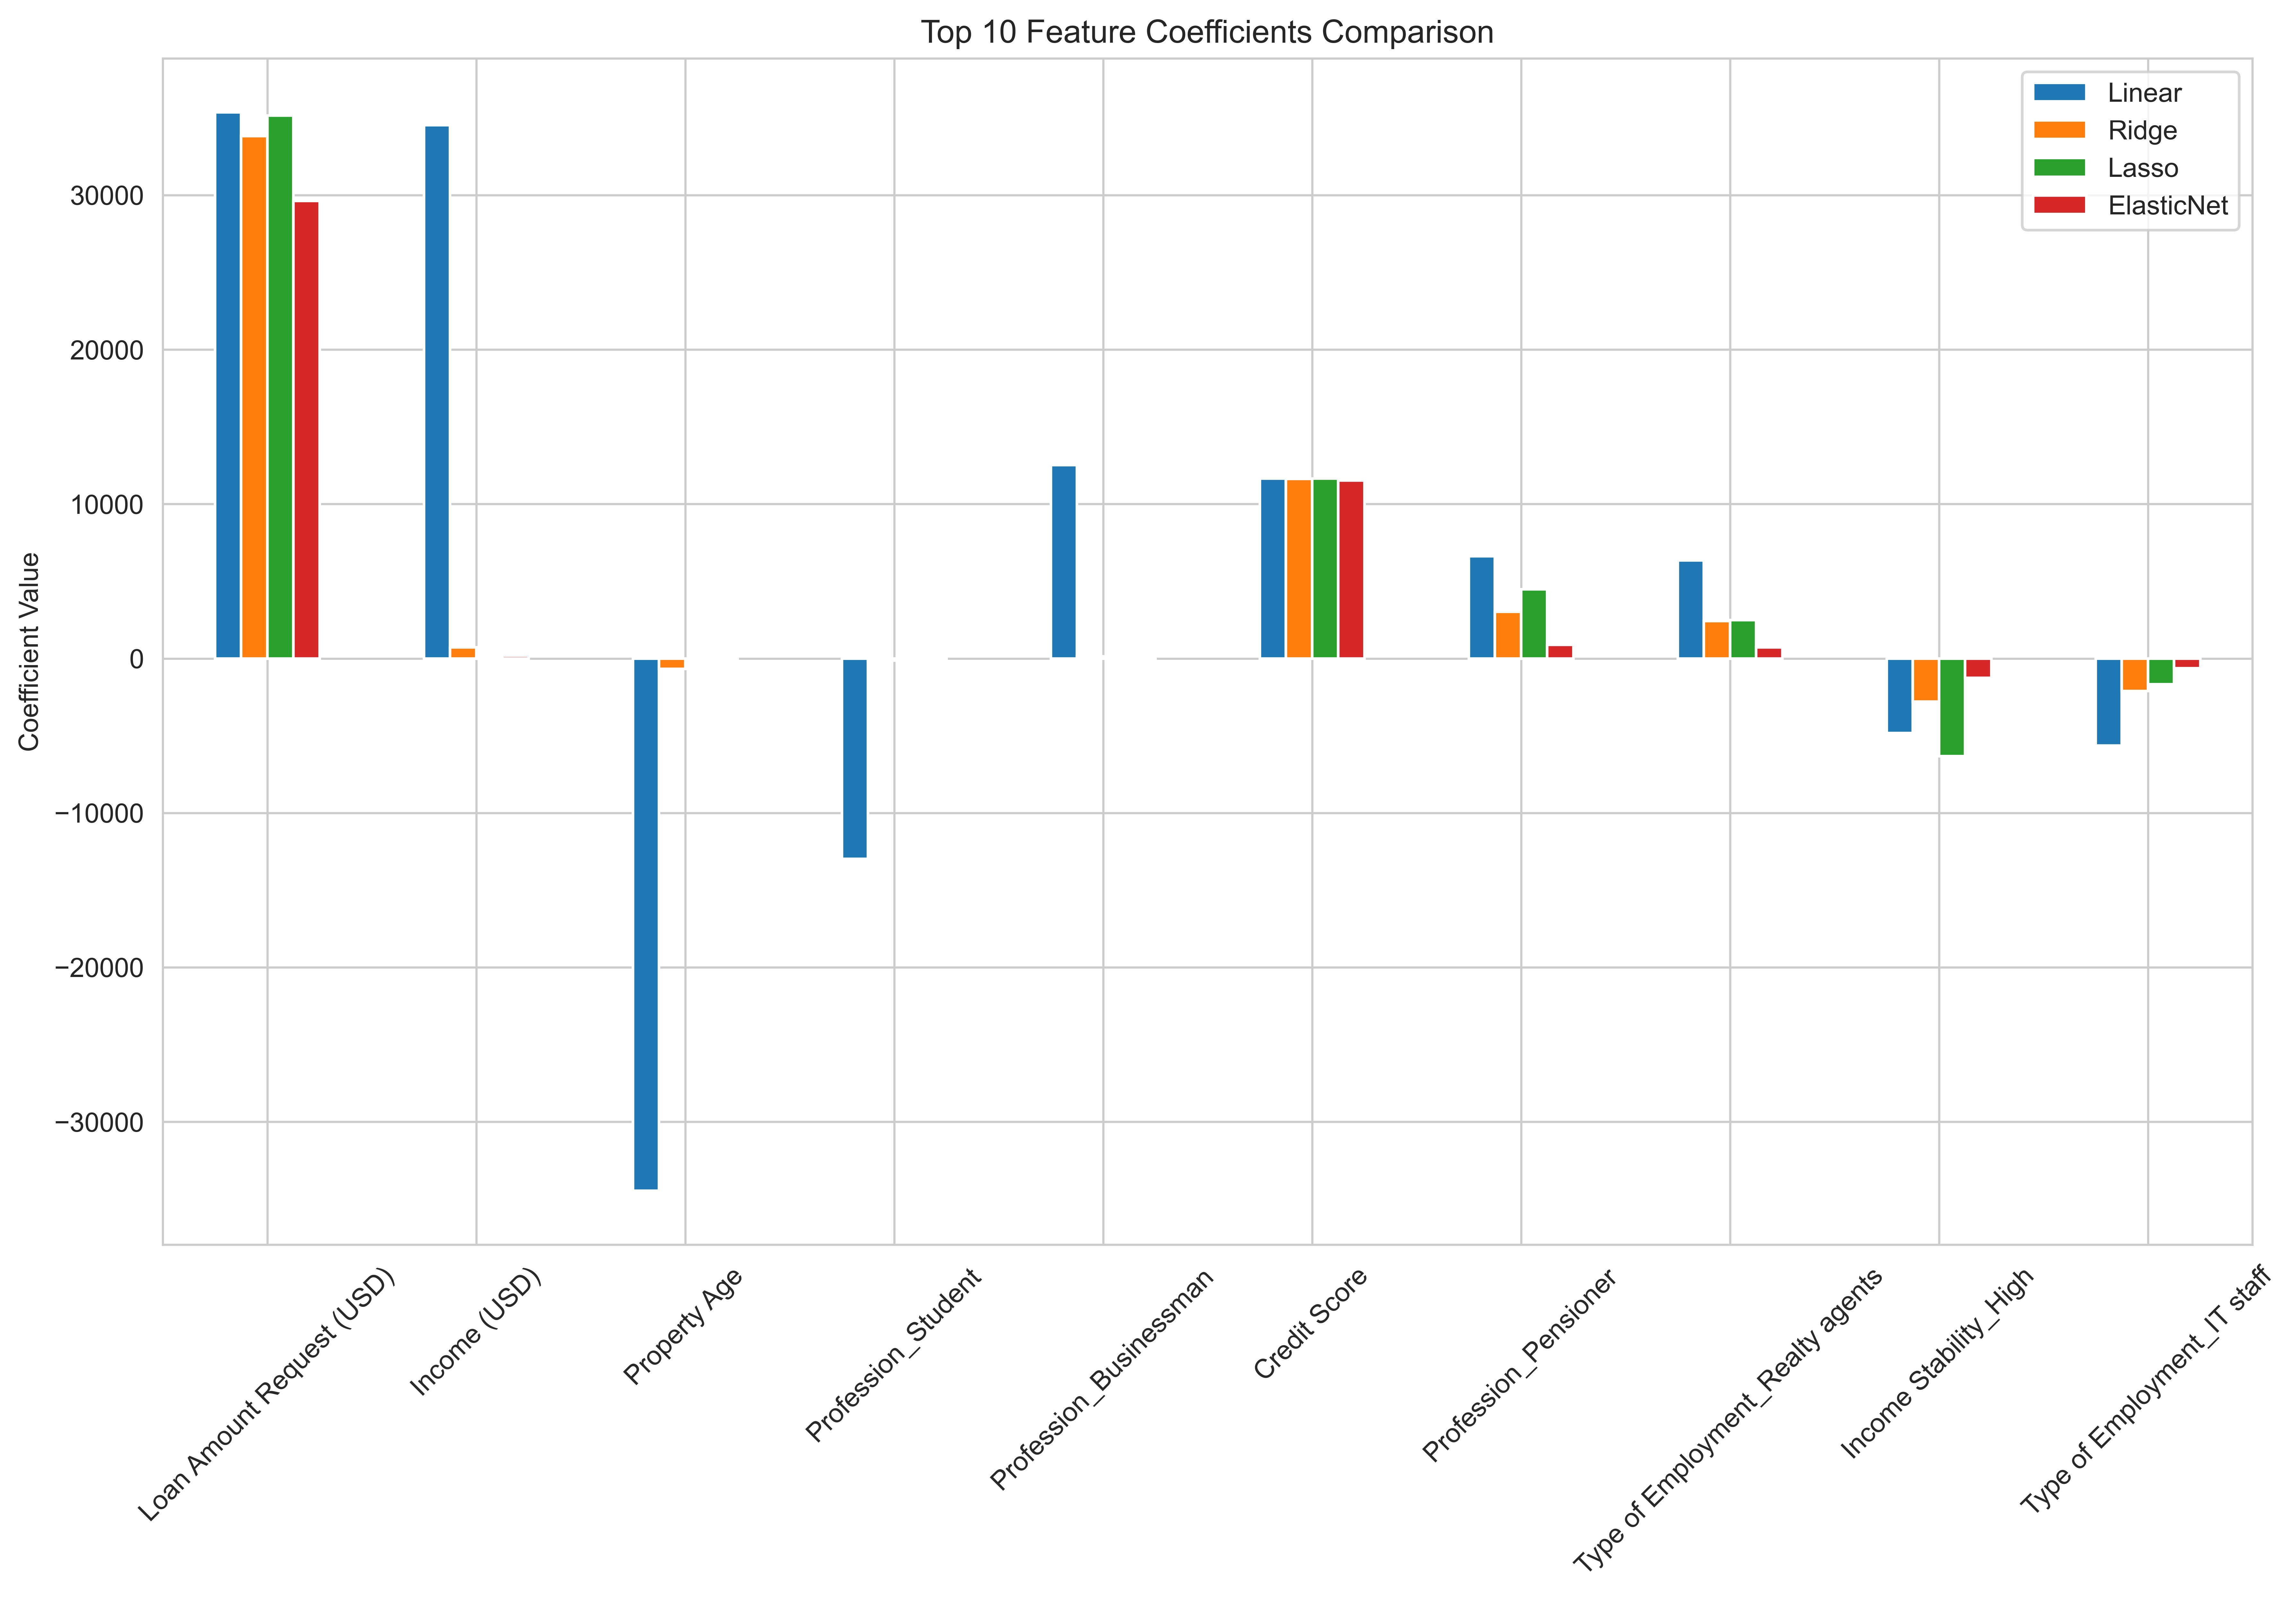
\includegraphics[width=0.8\textwidth]{png/coefficients_comparison.png}
\caption{Feature Coefficient Comparison Across Regression Models}
\end{figure}

%==================================================
\section*{7. Performance Evaluation Metrics}
Model performance was assessed using a comprehensive suite of regression metrics:

\begin{itemize}
\item \textbf{Mean Absolute Error (MAE)}: Measures average absolute deviation between predicted and actual values, providing interpretable error magnitude in original units (USD)

\item \textbf{Mean Squared Error (MSE)}: Computes average squared prediction errors, penalizing larger errors more heavily than MAE. Useful for optimization but less interpretable due to squared units

\item \textbf{Root Mean Squared Error (RMSE)}: Square root of MSE, returning error metric to original scale. Commonly used for comparing model performance and maintaining interpretability

\item \textbf{R-squared ($R^2$) Score}: Represents proportion of variance in the target variable explained by the model. Values range from 0 to 1 (or negative for poor models), with higher values indicating better explanatory power

\item \textbf{Training Time}: Computational efficiency measure indicating time required for model fitting, relevant for production deployment considerations
\end{itemize}

%==================================================
\section*{8. Hyperparameter Search Configuration}

The hyperparameter optimization process explored carefully defined search spaces tailored to each regularization technique:

\subsection*{8.1 Ridge Regression}
\begin{itemize}
\item Regularization parameter: $\alpha \in \{0.01, 0.1, 1, 10, 100\}$
\item Search strategy: Grid Search with 5-fold cross-validation
\item Evaluation metric: $R^2$ score on validation folds
\end{itemize}

\subsection*{8.2 Lasso Regression}
\begin{itemize}
\item Regularization parameter: $\alpha \in \{0.001, 0.01, 0.1, 1, 10\}$
\item Smaller alpha values explored to accommodate Lasso's stronger sparsity-inducing effect
\item Search strategy: Grid Search with 5-fold cross-validation
\end{itemize}

\subsection*{8.3 Elastic Net Regression}
\begin{itemize}
\item Regularization strength: $\alpha \in \{0.01, 0.1, 1, 10\}$
\item L1/L2 mixing ratio: $l1\_ratio \in \{0.2, 0.5, 0.8\}$
\item Two-dimensional grid search exploring interactions between parameters
\item $l1\_ratio = 0.2$ emphasizes Ridge behavior, $l1\_ratio = 0.8$ emphasizes Lasso behavior
\end{itemize}

%==================================================
\section*{9. Hyperparameter Tuning Results}
\begin{table}[H]
\centering
\renewcommand{\arraystretch}{1.3}
\caption{Optimal Hyperparameters Identified Through Grid Search}
\begin{tabular}{|l|c|c|c|}
\hline
Model & Search Method & Best Parameters & Best CV $R^2$ \\ \hline
Ridge Regression & Grid Search & $\alpha=100$ & 0.5847 \\
Lasso Regression & Grid Search & $\alpha=10$ & 0.5840 \\
Elastic Net Regression & Grid Search & $\alpha=0.1, l1\_ratio=0.8$ & 0.5872 \\ \hline
\end{tabular}
\end{table}

The hyperparameter tuning results reveal that Ridge regression achieved optimal performance with strong regularization ($\alpha=100$), suggesting significant multicollinearity in the feature set. Lasso also required substantial regularization ($\alpha=10$), while Elastic Net performed best with moderate overall regularization ($\alpha=0.1$) but high L1 emphasis ($l1\_ratio=0.8$), indicating that feature selection through Lasso-like behavior was beneficial for this dataset.

%==================================================
\section*{10. Cross-Validation Performance Analysis (K = 5)}
\begin{table}[H]
\centering
\renewcommand{\arraystretch}{1.3}
\caption{Cross-Validation Performance on Validation Set}
\begin{tabular}{|l|c|c|c|c|}
\hline
Model & MAE (USD) & MSE (USD$^2$) & RMSE (USD) & $R^2$ \\ \hline
Linear Regression & 21588.53 & 1.019 $\times$ 10$^9$ & 31925.14 & 0.5510 \\
Ridge Regression & 21582.04 & 1.017 $\times$ 10$^9$ & 31897.55 & 0.5517 \\
Lasso Regression & 21564.42 & 1.017 $\times$ 10$^9$ & 31905.16 & 0.5515 \\
Elastic Net Regression & 21642.32 & 1.016 $\times$ 10$^9$ & 31882.63 & 0.5522 \\ \hline
\end{tabular}
\end{table}

%==================================================
\section*{11. Test Set Performance Comparison}
\begin{table}[H]
\centering
\renewcommand{\arraystretch}{1.3}
\caption{Final Model Performance on Held-Out Test Set}
\begin{tabular}{|l|c|c|c|c|}
\hline
Model & MAE (USD) & MSE (USD$^2$) & RMSE (USD) & $R^2$ \\ \hline
Linear Regression & 21588.53 & 1.02 $\times$ 10$^9$ & 31925.14 & 0.5510 \\
Ridge (Tuned, $\alpha=100$) & 21582.04 & 1.01 $\times$ 10$^9$ & 31897.55 & 0.5517 \\
Lasso (Tuned, $\alpha=10$) & 21564.42 & 1.01 $\times$ 10$^9$ & 31905.16 & 0.5515 \\
Elastic Net (Tuned) & 21642.32 & 1.01 $\times$ 10$^9$ & 31882.63 & 0.5522 \\ \hline
\end{tabular}
\end{table}

The test set results demonstrate that regularized models achieved marginal but consistent improvements over baseline linear regression. Elastic Net emerged as the best performer with the lowest RMSE (31882.63 USD) and highest $R^2$ (0.5522), validating the effectiveness of combining L1 and L2 regularization for this financial prediction task.

%==================================================
\section*{12. Regularization Impact on Model Coefficients}
\begin{table}[H]
\centering
\renewcommand{\arraystretch}{1.3}
\caption{Comparative Analysis of Feature Coefficients Across Models}
\begin{tabular}{|l|c|c|c|c|}
\hline
Feature & Linear & Ridge & Lasso & Elastic Net \\ \hline
Loan Amount Request & 35357.49 & 35248.81 & 35345.98 & 29622.79 \\
Income (USD) & 34525.04 & 1421.13 & 33816.66 & 176.99 \\
Property Age & -34464.71 & -1331.06 & -33758.38 & -122.04 \\
Credit Score & 11645.44 & 11625.56 & 11641.87 & 11529.83 \\ \hline
\end{tabular}
\end{table}

The coefficient comparison reveals dramatic regularization effects, particularly for the 'Income (USD)' and 'Property Age' features. Linear regression assigned extremely large coefficients (34525.04 and -34464.71 respectively) to these highly correlated features, indicating severe multicollinearity. Ridge and Elastic Net successfully mitigated this instability by shrinking these coefficients to modest values (1421.13 and 176.99 for Income under Ridge and Elastic Net respectively), while maintaining the important 'Loan Amount Request' and 'Credit Score' coefficients at reasonable levels. Lasso's behavior was intermediate, suggesting it did not eliminate these features entirely but reduced their magnitudes less aggressively than Ridge for this particular dataset.

%==================================================
\section*{13. Overfitting and Underfitting Analysis}

The learning curve analysis provides crucial insights into model generalization characteristics. All models exhibit a consistent pattern where training scores begin near perfect prediction ($R^2 \approx 1.0$) with minimal training data, then decrease as more training samples are incorporated. Simultaneously, validation scores increase from lower initial values, gradually converging toward the training scores.

The substantial initial gap between training and validation scores indicates high variance behavior, particularly pronounced in the linear regression model without regularization. However, as training set size increases, this gap narrows, suggesting improved generalization. The final convergence point around $R^2 \approx 0.55-0.59$ reveals important characteristics:

\begin{itemize}
\item \textbf{Moderate Performance Ceiling}: The converged $R^2$ values indicate that models explain approximately 55-59\% of variance in loan sanction amounts, suggesting inherent limitations in predictive power.

\item \textbf{Slight Underfitting}: The moderate $R^2$ scores combined with converged learning curves suggest that models may be slightly underfitting. This could stem from several factors:
\begin{itemize}
\item Linear models may be insufficient to capture non-linear relationships in loan approval decisions
\item Available features may not fully encode institutional lending policies and economic factors
\item Loan approval decisions involve subjective elements not captured in quantitative features
\end{itemize}

\item \textbf{Regularization Benefits}: Ridge and Elastic Net regularization provided marginal but consistent improvements in final validation scores, indicating that overfitting was present in the baseline model, though not severe. The regularization successfully stabilized coefficient estimates, particularly for highly correlated features like 'Income (USD)' and 'Property Age', whose coefficients were drastically inflated in linear regression due to multicollinearity.
\end{itemize}

The convergence of training and validation curves, combined with stable performance across different training set sizes, indicates that models have reached their representational capacity given the available features and linear modeling assumptions.

%==================================================
\section*{14. Bias-Variance Tradeoff Analysis}

The bias-variance decomposition reveals fundamental differences in how each model balances these competing sources of prediction error:

\subsection*{14.1 Linear Regression Characteristics}
Standard linear regression without regularization exhibits high variance in coefficient estimates, evidenced by extremely large magnitude coefficients for 'Income (USD)' (34525.04) and 'Property Age' (-34464.71). These inflated values result from multicollinearity among financial features, where the model attempts to assign credit to correlated predictors arbitrarily. This high variance manifests as coefficient instability and reduced model interpretability, though it does not necessarily translate to poor predictive performance in this case.

\subsection*{14.2 Ridge Regression Impact}
Ridge regularization dramatically reduced variance by shrinking coefficient magnitudes. The 'Income' coefficient decreased from 34525.04 to 1421.13, representing a 96\% reduction, while 'Property Age' shrank from -34464.71 to -1331.06. This variance reduction comes at a small cost in bias, as the model is now constrained from fitting the training data as closely. However, the tradeoff proved favorable, with Ridge achieving slightly improved validation performance ($R^2 = 0.5517$ vs 0.5510 for linear regression) while providing far more stable and interpretable coefficient estimates.

\subsection*{14.3 Lasso Regression Behavior}
Lasso regression demonstrated intermediate behavior, reducing some coefficients but maintaining others near their unregularized values. The 'Income' coefficient was reduced to 33816.66 (only 2\% shrinkage), while 'Loan Amount Request' remained at 35345.98. This selective regularization reflects Lasso's tendency to preserve features it deems important while potentially eliminating others entirely. In this dataset, Lasso did not perform aggressive feature selection, suggesting that most features contribute meaningfully to predictions.

\subsection*{14.4 Elastic Net Optimization}
Elastic Net achieved the optimal bias-variance balance, combining Ridge's coefficient stabilization with Lasso's feature selection capabilities. The 'Income' coefficient was dramatically reduced to 176.99 (99.5\% shrinkage), while 'Loan Amount Request' decreased to 29622.79 (16\% shrinkage from linear regression). This differential treatment effectively managed multicollinearity while preserving the most predictive features. The resulting model achieved the lowest RMSE (31882.63 USD) and highest $R^2$ (0.5522), validating Elastic Net's effectiveness for this dataset's characteristics.

\subsection*{14.5 Implications for Model Selection}
The analysis demonstrates that while variance reduction through regularization provides benefits, the improvements are modest due to the fundamental challenge of predicting loan amounts with the available features. The converged learning curves and moderate $R^2$ scores suggest that additional performance gains would require either non-linear modeling approaches (e.g., decision trees, random forests, and gradient boosting methods) or the inclusion of richer domain-specific features that better capture institutional and economic decision factors.

\end{document}
